% $File: report.tex
% $Date: Sun Nov 16 13:51:14 2014 +0800

\documentclass {beamer}
%\usetheme{JuanLesPins}
\usetheme{Copenhagen}
\setbeamertemplate{itemize items}[ball]
\setbeamercovered{transparent}
\setbeamertemplate{itemize subitem}[circle] % if you wnat a circle
\setbeamertemplate{blocks}[rounded][shadow=true]
%\usetheme[height=7mm]{Rochester}
\useoutertheme{infolines}
\usepackage{fontspec,amsmath,amssymb,zhspacing,verbatim}
\usepackage[backend=biber]{biblatex}


\let\Oldsum\sum
\renewcommand{\sum}{\displaystyle\Oldsum}
\let\Oldprod\prod
\renewcommand{\prod}{\displaystyle\Oldprod}

\theoremstyle{plain}

\usepackage[absolute,overlay]{textpos}
\newenvironment{reference}[2]{%
  \begin{textblock*}{\textwidth}(#1,#2)
      \footnotesize\it\bgroup\color{red!50!black}}{\egroup\end{textblock*}}

\zhspacing

\setbeamertemplate{footline} {
  \leavevmode%
  \hbox{%
    \begin{beamercolorbox}[wd=\paperwidth,ht=2.25ex]{corporatecolor}
      \begin{beamercolorbox}[wd=.333333\paperwidth,ht=2.25ex,dp=1ex,center]{author in head/foot}%
        \usebeamerfont{author in head/foot}
        \insertshortauthor
      \end{beamercolorbox}%
      \begin{beamercolorbox}[wd=.333333\paperwidth,ht=2.25ex,dp=1ex,center]{title in head/foot}%
        \usebeamerfont{title in head/foot}
        \insertshorttitle
      \end{beamercolorbox}%
      \begin{beamercolorbox}[wd=.333333\paperwidth,ht=2.25ex,dp=1ex,right]{date in head/foot}%
        \usebeamerfont{date in head/foot}\insertshortdate{}\hspace*{2em}
        \insertframenumber{} / \inserttotalframenumber\hspace*{2ex}
      \end{beamercolorbox}
    \end{beamercolorbox}
  }%
  \vskip0pt%
}

\title{Let Music Roll}
\subtitle{HackShanghai}
\author {Team: \textbf{blxlrsmb}}
\institute{
  Department of Computer Science and Technology\\
  Tsinghua University\\
}
\date{Nov 16, 2014}

\begin{document}

\frame[plain]{\titlepage }

%\begin{frame}{Overview}
%\end{frame}

%\begin{frame}{Content}
%\tableofcontents
%\end{frame}

%File: q1.tex
%Date: Sun Nov 16 14:11:57 2014 +0800
%Author: Yuxin Wu <ppwwyyxxc@gmail.com>

\section{Introduction}
\begin{frame}
\begin{exampleblock}{\textbf{Project}}
Music understanding and visualization.
\end{exampleblock}

\begin{figure}[H]
  \centering
  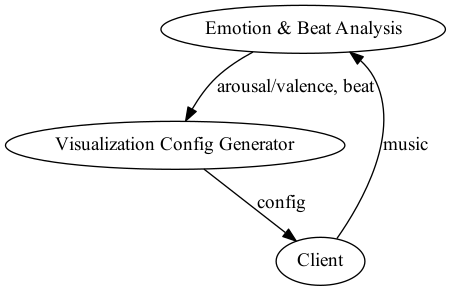
\includegraphics[width=0.7\textwidth]{res/illu.dot.png}
\end{figure}


\end{frame}

\section{Backend Algorithms}
\begin{frame}{Beat Detection}
\begin{enumerate}
    \item Separate \textbf{percussive} and \textbf{harmonic}:
      \begin{enumerate}
        \item Short-time Fourier Transform
        \item Harmonic Percussive Source Separation
        \item Inverse Short-time Fourier Transform
      \end{enumerate}
    \item Detect exact beats from percussive: local estimation with global regularization
  \end{enumerate}
\end{frame}

\begin{frame}{Emotion Detection - Features}
\begin{enumerate}[(a)]
    \item Root Mean Square
    \item High Quefreqncy Log Frequency Spectrum
    \item Chromagram
    \item High Quefrency Chomagram
    \item Mel-frequency Cepstrum
    \item Low Quefrency Log Frequency Spectrum
    \item Log Frequency Spectrum
    \item dbPower
    \item Low Frequency Power
\end{enumerate}
\end{frame}

\begin{frame}{Emotion Detection - Data \& Model}
       \textbf{"Emotion in Music 2014"} public dataset.

     Trained with \textbf{Gradient Boosting Trees(GBT)} on 2.8G data.

     Predict Arousal/Valence of music segments with high accuracy.
\begin{figure}[H]
  \centering
  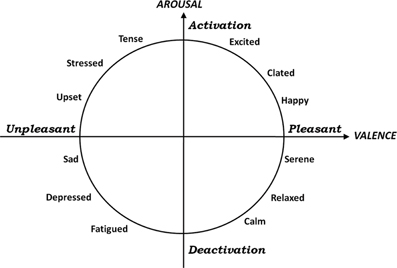
\includegraphics[width=0.6\textwidth]{res/av.jpg}
\end{figure}

\end{frame}

\section{Frontend}
\begin{frame}{3D Tour}
     Use pre-defined visualizations from Light.js/Three.js.

     Show arousal/valence values with HighCharts.js.

     Synchronize with the music using backend analysis results.

Totally differ from old-fashioned music visualization:
\begin{figure}[H]
  \centering
  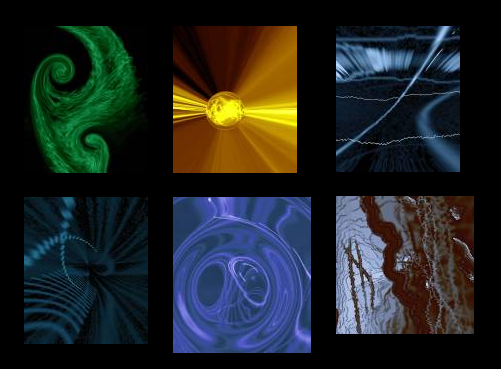
\includegraphics[width=0.6\textwidth]{res/out.png}
\end{figure}

\end{frame}

%\input{q2.tex}
%\input{q3.tex}
%\input{q4.tex}
%\input{trick.tex}



\begin{frame}{}
  \begin{center}
  \Huge Demo!
\end{center}
\end{frame}

\end{document}

